\chapter{Systemdesign og bølgelængdevalg}
\label{chap:system_design}

\section{Overordnet designstrategi}

Systemdesignet blev udviklet ud fra en kombination af litteratur, optisk teori og praktiske komponenthensyn. Som udgangspunkt blev \SI{660}{nm} og \SI{940}{nm} valgt, da disse bølgelængder ligger tæt på de klassiske bølgelængdeområder anvendt i mange kommercielle og kliniske pulsoximetre \cite[s.~35]{Webster1997}. Valget er motiveret af, at rødt lys omkring \SI{660}{nm} giver høj absorptionskontrast mellem oxyhæmoglobin og deoxyhæmoglobin, mens nær-infrarødt lys omkring \SI{940}{nm} generelt har større penetration i væv og samtidig indgår i det klassiske to-bølgelængdeprincip for pulsoximetri.

Valget blev desuden understøttet af komponenttilgængelighed, da relevante LED'er er let tilgængelige som standardkomponenter, og deres databladsspecifikationer er veldokumenterede. Dette gjorde dem velegnede som udgangspunkt for det analoge system.

Efter det indledende designvalg blev bølgelængderne undersøgt yderligere ved hjælp af både spektrometriske og hyperspektrale målinger. Disse målinger blev ikke anvendt til at vælge de første kandidatbølgelængder, men til at verificere lyskildernes faktiske spektrale placering og til at vurdere den relative transmission gennem fingervæv ved udvalgte bølgelængder.

Verificeringen er vigtig, da LED'ers faktiske peak-bølgelængde kan afvige fra den bølgelængde, der er angivet i databladet. Litteraturen beskriver både LED-afvigelser på op til omtrent $\pm\SI{15}{nm}$ og væsentlige afvigelser fra de klassiske \SI{660}{nm}- og \SI{940}{nm}-områder i praktiske pulsoximetre \cite[s.~35]{Webster1997} \cite{Ruberry2025}.

\paragraph{Spektrometer.}
Et spektrometer anvender dispersion, typisk via et diffraktionsgitter, til at adskille indkommende lys i dets spektrale komponenter. Herved kan intensiteten som funktion af bølgelængde bestemmes.

Spektrometeret blev anvendt som et valideringsværktøj til at bestemme de faktiske emissionsspektre for LED-kandidaterne, sammenligne dem med et kommercielt pulsoximeter og undersøge, hvilke spektrale områder der kunne transmitteres gennem fingeren.

\paragraph{Hyperspektralt setup.}

Målingerne fra det hyperspektrale setup blev anvendt til at sammenligne den relative transmitterede intensitet ved forskellige bølgelængder under den givne optiske geometri. Resultaterne blev dermed brugt som en supplerende vurdering af, hvilke bølgelængdeområder der var interessante til videre brug i pulsoximetrisystemet.

\section{Valg af bølgelængder}
\label{sec:wavelength_selection}

Ud over de to hovedbølgelængder blev \SI{810}{nm} og \SI{970}{nm} undersøgt som supplerende kandidatbølgelængder. \SI{810}{nm} er interessant som et omtrent isosbestisk punkt, mens \SI{970}{nm} blev inkluderet som en supplerende NIR-kandidat, da området ligger tæt på \SI{940}{nm}, men kan give anden transmission gennem væv og anden LED-/detektorrespons. Disse bølgelængder blev karakteriseret spektrometrisk, men blev ikke integreret i det endelige analoge system på grund af tidsbegrænsninger.

\begin{table}[h]
\centering
\caption{Oversigt over undersøgte kandidatbølgelængder og deres rolle i projektet.}
\label{tab:kandidat_boelgelaengder}
\renewcommand{\arraystretch}{1.2}
\begin{tabularx}{\textwidth}{l l X X}
\toprule
Kandidatbølgelængde & Rolle & Motivation & Status i projektet \\
\midrule
\SI{660}{nm} & Rød hovedmåling & Høj absorptionsforskel mellem HbO$_2$ og Hb & Brugt i analogt system, karakteriseret med spektrometer \\
\SI{810}{nm} & Isosbestisk reference & Omtrent samme absorption for HbO$_2$ og Hb & Karakteriseret med spektrometer \\
\SI{940}{nm} & IR-hovedmåling & Klassisk NIR-bølgelængde med større vævspenetration og komplementær information til \SI{660}{nm} & Brugt i analogt og hyperspektralt system og karakteriseret med spektrometer  \\
\SI{970}{nm} & Supplerende NIR-måling & Ekstra sammenligning i det nær-infrarøde område & Karakteriseret med spektrometer \\
\bottomrule
\end{tabularx}
\end{table}


\section{Systemarkitektur}

Som vist i figur \ref{fig:blockdiagram_architecture} styres LED'erne via et separat driverkredsløb. Da de røde og infrarøde LED'er har forskellige fremadspændinger og ønskede drivstrømme, blev driveren designet således, at strømmen til hver LED kan tilpasses ved hjælp af udskiftelige modstande. En N-kanal MOSFET anvendes som switch, så LED-strømmen kan leveres fra et separat \SI{9}{V} batteri frem for direkte fra AD3'ens udgange.

De multipleksede LED'er er monteret i et 3D-printet kabinet, hvor de belyser fingeren i transmissionsgeometri. Det transmitterede lys detekteres af en S1223-fotodiode placeret på den modsatte side af fingeren. Fotodiodens strøm føres herefter til transimpedansforstærkeren, hvor den omsættes til en spænding.

Den oprindelige analoge signalkæde blev designet med TIA, lavpasfilter, højpasfilter og gain-trin. I den endelige måleprocedure blev DC-informationen dog bevaret til beregning af $\frac{AC}{DC}$, hvorfor højpasfilteret ikke indgik i den endelige SpO$_2$-analyse.

Som dataopsamlingsenhed blev et Analog Discovery 3 anvendt. Denne enhed blev brugt både til at generere styresignaler til tidsmultipleksing af LED'erne og til at opsamle det analoge signal fra signalkæden. Den endelige signalbehandling og visualisering blev udført i Python.

\begin{figure}[htbp]
    \centering
    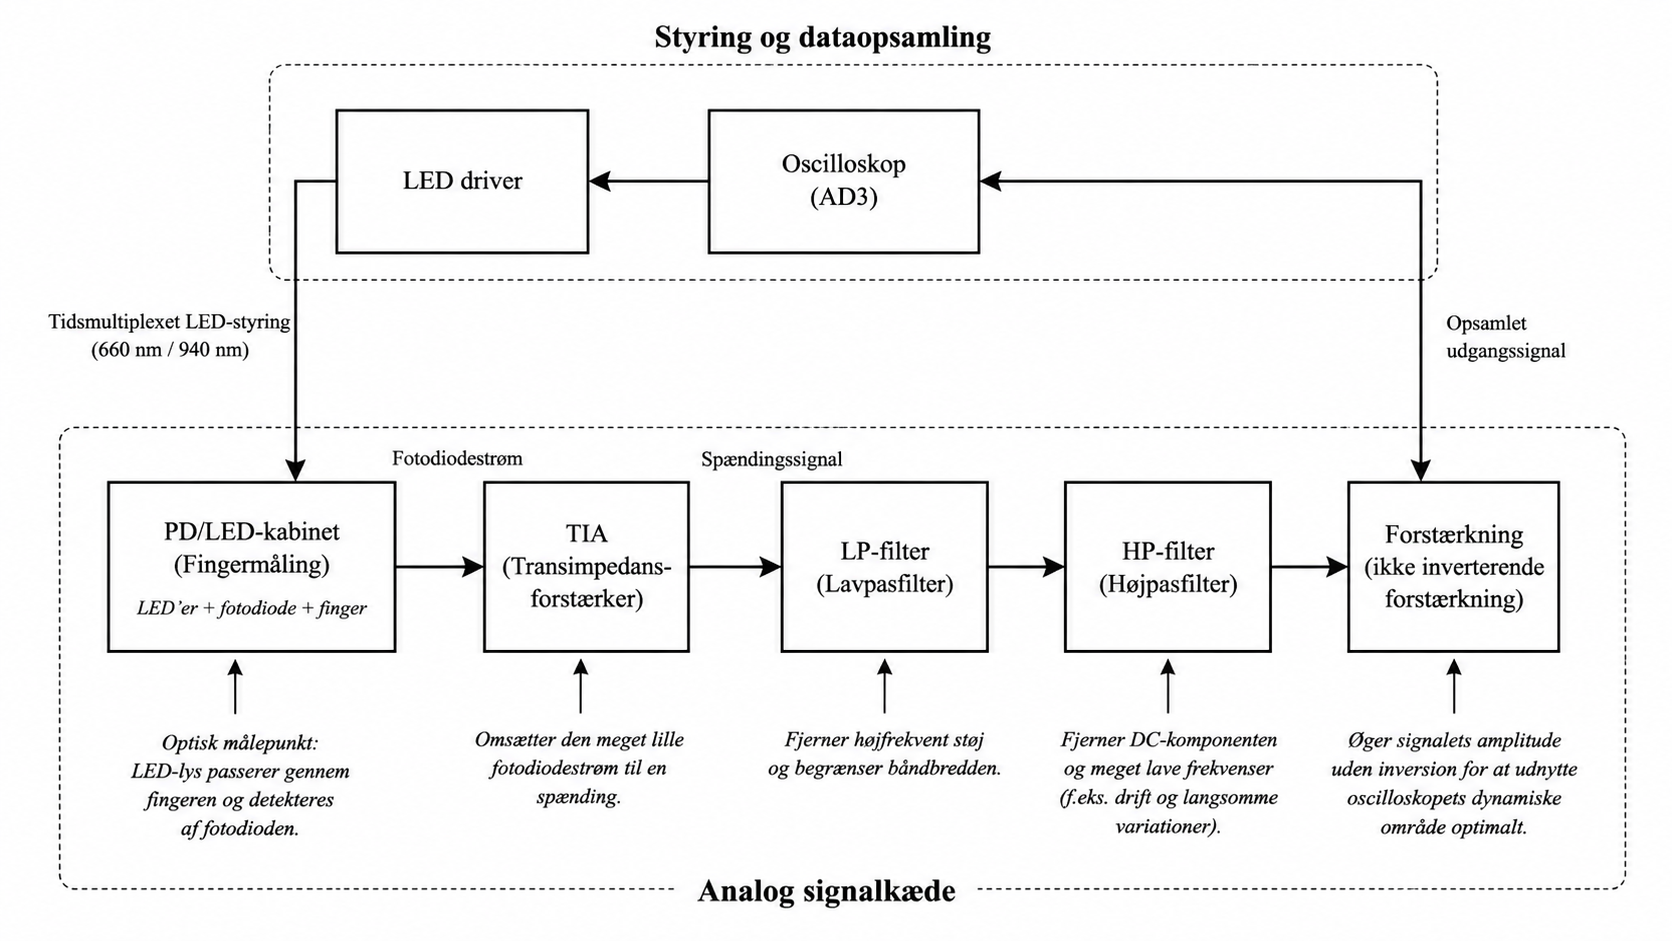
\includegraphics[width=1\textwidth]{Pictures/Graphs/blockdiagram_architecture.png}
    \caption{Overordnet systemarkitektur for det udviklede pulsoximetersystem, fra LED-driver og fingerhylster til analog signalbehandling, dataopsamling og analyse i Python.}
    \label{fig:blockdiagram_architecture}
\end{figure}


\section{Mekanisk design}
\label{sec:mechanical_design}

\subsection{Modulært 3D-printet design}

\paragraph{Modularitet.} Det 3D-printede design set i figur \ref{fig:3D design arkitektur} blev valgt for at understøtte modularitet og hurtig prototyping. Hvert stadie er monteret på en puslespils-lignende brik, der forbindes til de øvrige via dovetail-/puslespilsinspirerede samlinger. Dette tillader moduler der kan opgraderes, fjernes og tilføjes uden at hele systemet skal ombygges, hvilket er en kritisk egenskab under prototyping.

Det giver muligheder som at f.eks. tilføje et evt. \SI{50}{Hz} notch-filter i signalkæden hvis det viser sig at \SI{50}{Hz} støj dominerer.

Derudover er PLA og PETG elektrisk isolerende materialer. Det reducerer risikoen for utilsigtede kortslutninger, hvis printede kredsløb eller loddepunkter kommer tæt på ledende overflader som et optisk bord.

\begin{figure}[htbp]
    \centering
    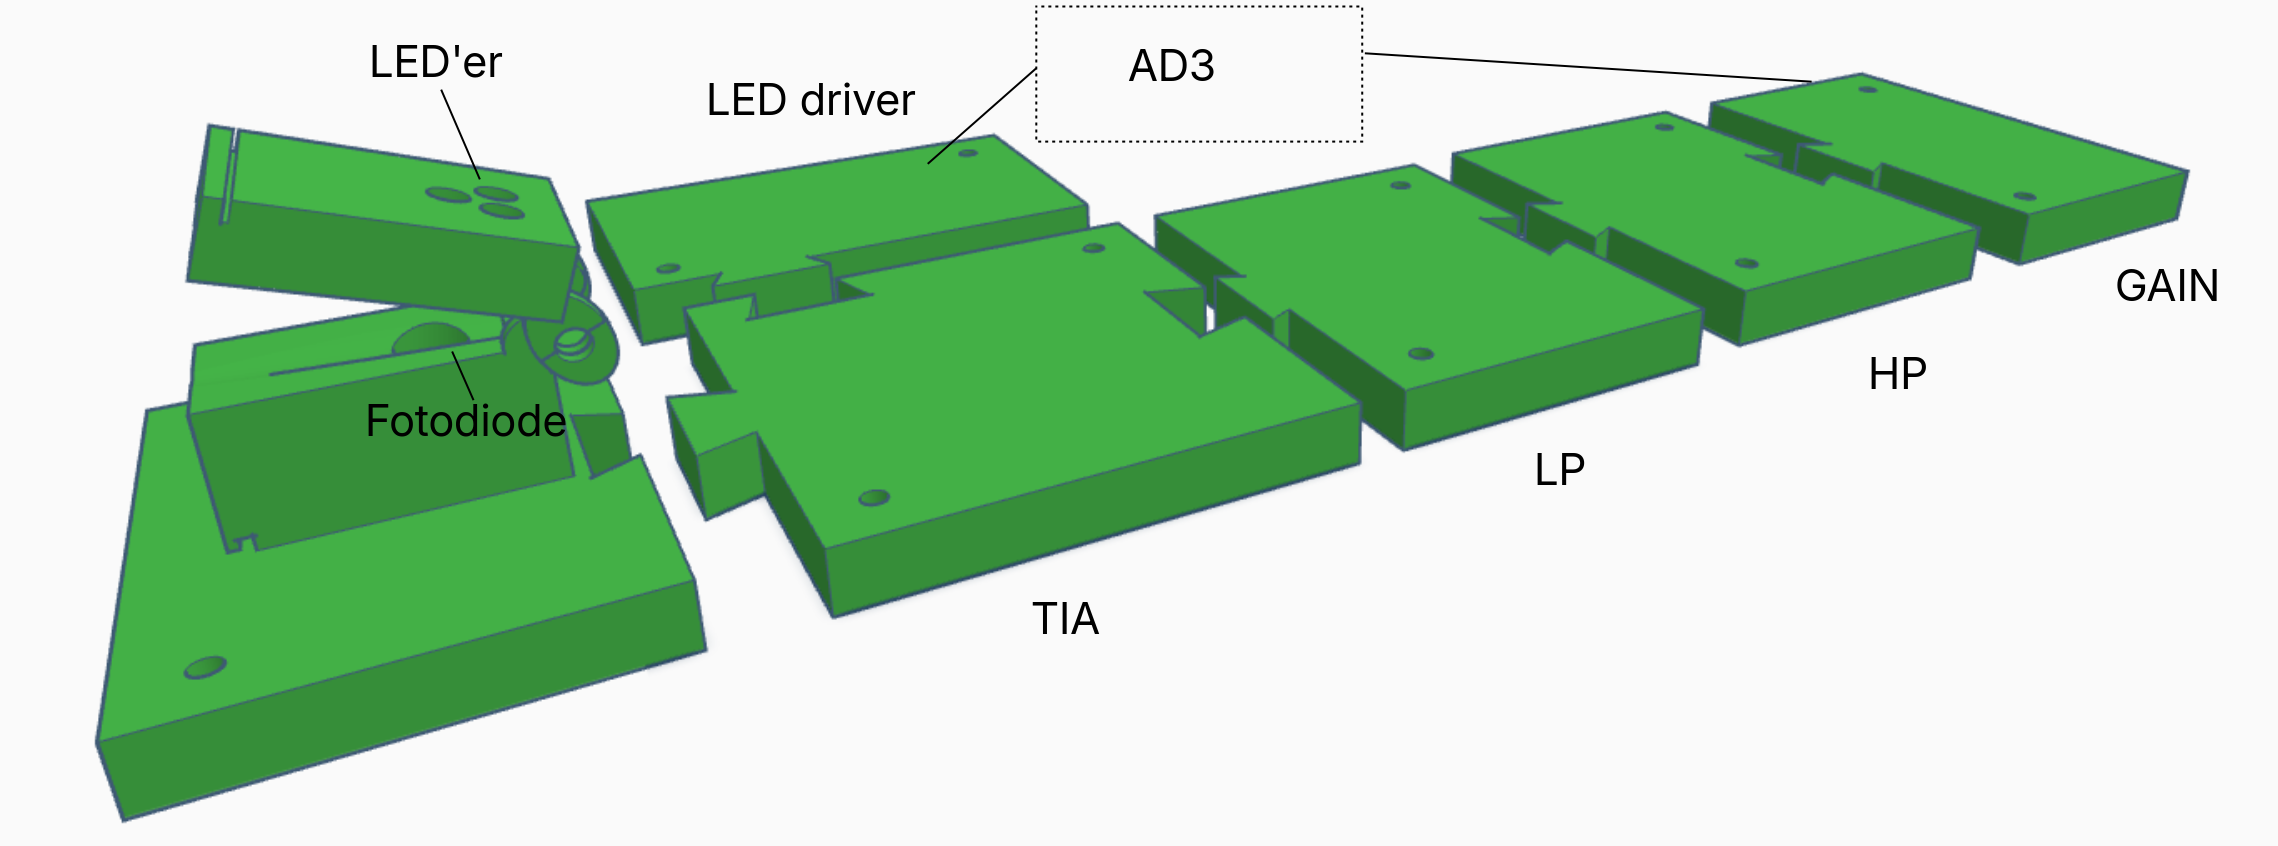
\includegraphics[width=1\textwidth]{Pictures/Other/3D print kæde.png}
    \caption{3D design af systemarkitektur. Farverne i CAD-modellen er kun anvendt for visuel adskillelse. De tre LED-positioner blev oprindeligt designet til \SI{660}{nm}, \SI{810}{nm}, \SI{940}{nm}. I det endelige analoge system blev kun \SI{660}{nm} og \SI{940}{nm} implementeret.}
    \label{fig:3D design arkitektur}
\end{figure}

\begin{figure}[htbp]
    \centering
    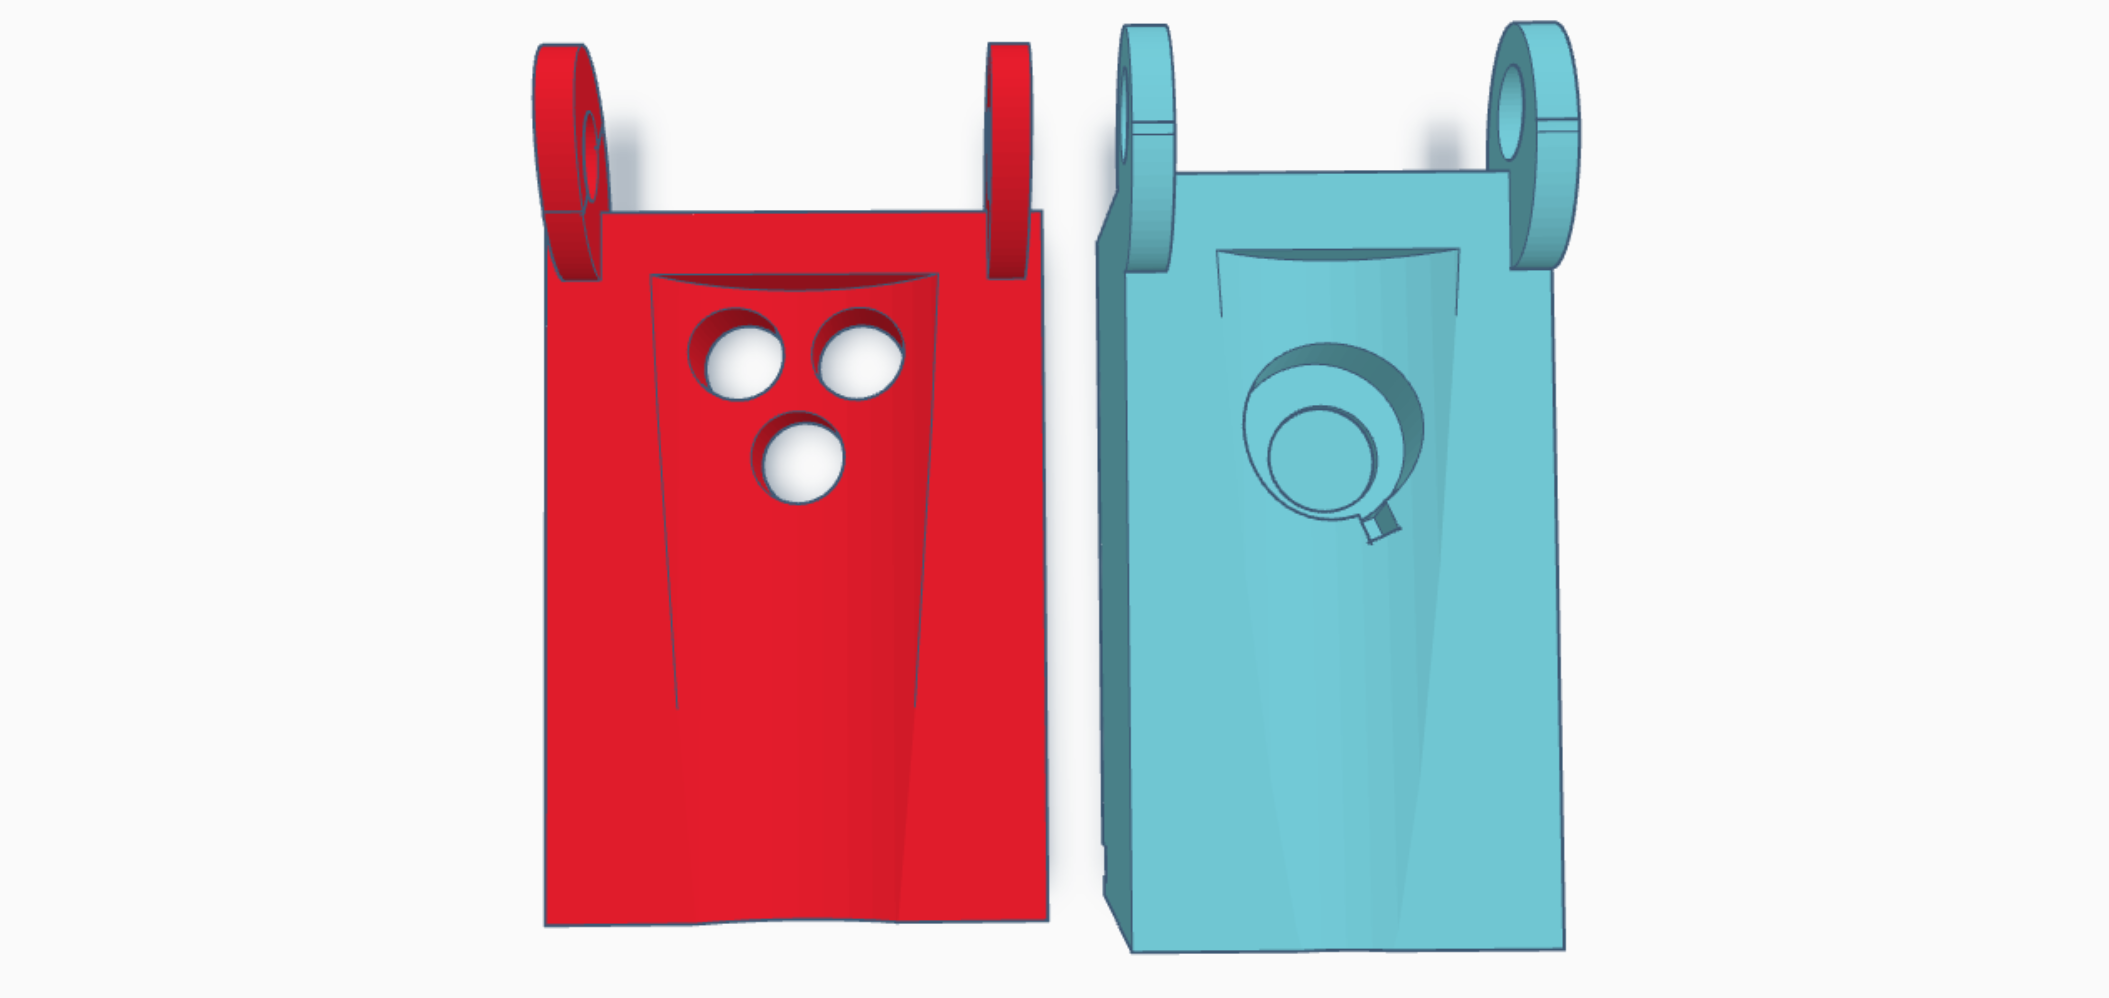
\includegraphics[width=1\textwidth]{Pictures/Other/LED PD closeup.png}
    \caption{CAD-udsnit af fingerhylsteret med top- og bunddel. LED'er og fotodiode er placeret på hver sin side af fingeren, så målingen udføres i transmissionsgeometri. De to halvdele er forbundet via en cylindrisk låsepin.}
    \label{fig:3D design finger hylster}
\end{figure}

\subsection{Praktiske designhensyn}

\paragraph{Omgivelseslys og optisk shunting.} Hylsteret blev designet til at reducere indkobling af omgivelseslys i fotodioden. Litteraturen anbefaler, at pulsoximeterprober udføres i sort, uigennemsigtigt materiale eller indkapsles i et uigennemsigtigt hus, så uønskede lysveje begrænses \cite[s.~185]{Webster1997}. Et relateret problem er optisk shunting, hvor lys kan nå detektoren uden at have passeret den ønskede vævsvej \cite{Ruberry2025}.

\paragraph{Pulsoxi-hylster.} Som set i figur \ref{fig:3D design finger hylster} er der specielt designet plads til fotodioden og de to LED'er. De specifikke mål er hentet fra hvert datablad og itereret over med de faktiske mål for komponenterne.

Komponenterne blev fastgjort mekanisk, så limen ikke lå i den optiske strålegang eller skabte elektrisk kontakt mellem benene.

Der blev desuden indarbejdet en fingerformet rille i både top- og bundsektionen for at forbedre fingerens placering og reproducerbarheden af målegeometrien. Geometrien blev lavet ud fra en repræsentativ fingerstørrelse og er derfor ikke nødvendigvis optimal for alle brugere.

Under samling blev fingerhylsterets geometri justeret, da direkte kontakt mellem fingerblommen og S1223-fotodioden gav et stort støjsignal ud af TIA'en. Ved at hæve hylstergeometrien lokalt og øge afstanden mellem fingerblomme og fotodiode forsvandt den observerede støj.

\paragraph{JST-forbindelser.} JST-XH-forbindelser blev anvendt for at gøre modulerne aftagelige og for at lette fejlfinding, ombygning og udskiftning af delkredsløb. Med JST-kabler kan man selv bestemme længden af kablerne. Forbindelserne sidder godt fast med en simpel låsemekanisme, og de er billige.

\section{Elektronisk design}
\label{sec:electrical_design}

\subsection{LED-driver}

LED-driverstadiet blev adskilt fra resten af signalkæden for at reducere kobling af switching-transienter ind i det følsomme analoge målekredsløb og for at levere LED-strømmen fra en separat forsyning. AD3'ens digitale udgange blev anvendt via pattern generatoren, så LED'erne kunne pulseres i en fast sekvens. De digitale udgange er beregnet til logiksignaler og har en begrænset udgangsstrøm, se figur \ref{fig:ad3_datasheet} i appendiks. De blev derfor kun anvendt som styresignaler til MOSFET-gatene, mens selve LED-strømmen blev leveret fra et separat \SI{9}{V}-batteri. For at definere MOSFET'ens gate-source-spænding blev AD3'ens GND og batteriets GND forbundet.

Hver LED drives gennem en 2N7000 N-kanal MOSFET konfigureret som en low-side switch. Det digitale styresignal fra AD3'en, \SIrange{0}{3.3}{V}, styrer MOSFET'ens gate, mens drain er forbundet til LED-katoden via en udskiftelig strømbegrænsende seriemodstand $R_{LED}$ og source til GND. LED-anoden tilsluttes den positive terminal på \SI{9}{V}-batteriet. LED-strømmen kan approksimeres som
\begin{equation}
    I_{LED} = \frac{V_{CC} - V_f - V_{DS(\text{on})}}{R_{LED}},
    \label{eq:led_current}
\end{equation}
hvor $V_f$ er LED'ens fremadspænding, og $V_{DS(\text{on})}$ er spændingsfaldet over MOSFET'en i ledende tilstand. Dette spændingsfald afhænger af gate-source-spændingen $V_{GS}$ og den valgte LED-strøm, og blev derfor behandlet som et praktisk tab.

For at vurdere om 2N7000 var egnet som switch, blev datasheetets transfer-karakteristik og on-resistance-karakteristik anvendt, se figur \ref{fig:2N7000_transfer_karakteristik} og figur \ref{fig:2N7000_onresistance} i appendiks. Transfer-karakteristikken viser sammenhængen mellem gate-source-spænding $V_{GS}$ og drain-strøm $I_D$, mens on-resistance-karakteristikken viser MOSFET'ens modstand i ledende tilstand, $R_{DS(\text{on})}$. Graferne blev brugt som en praktisk kontrol af, at transistoren kunne lede strømme i den ønskede størrelsesorden ved et gate-signal på \SI{3.3}{V}.

Gate-threshold-spændingen blev ikke brugt som eneste designkriterium, da den kun angiver hvornår transistoren begynder at lede, ikke hvornår den fungerer som en god switch. I stedet blev MOSFET'ens spændingsfald behandlet som et praktisk tab i LED-strømligningen, svarende til leddet $V_{DS(\text{on})}$ i ligning \ref{eq:led_current}. Da LED-strømmen samtidig begrænses af en seriemodstand, vil mindre variationer i MOSFET'ens on-resistance primært give en mindre ændring i den faktiske LED-strøm.

MOSFET'ens switching-tid ligger i ns-området og er dermed væsentligt kortere end de anvendte målevinduer i tidsmultipleksingen. Switchinghastigheden blev derfor ikke vurderet som den begrænsende faktor i systemet. Den praktiske begrænsning lå i stedet i analog settling og den valgte tidsmultipleksing.


\subsection{Transimpedansforstærker - TIA}

TIA'en er baseret på en OP27G, som er en lavstøjs præcisionsoperationsforstærker. TIA'en er vist i figur \ref{fig:PD_ingen_bias_TIA}, og er også vist i PCB-skemaet i figur \ref{fig:TIA_LP} i appendiks.

OP27G er ikke en FET-input-opamp. Dermed følger designet ikke den typiske anbefaling om FET-input i meget højimpedante fotodiode-TIA'er, hvor lav input-biasstrøm er en fordel \cite[s.~81]{Webster1997}. Komponenten blev anvendt, fordi den var tilgængelig i projektet og gav et brugbart proof-of-concept-signal.

I feedback-stien fra $V_{out}$ til operationsforstærkerens inverterende indgang $-in$ er der en modstand, betegnet med $R_f$, der sætter transimpedansen, dvs. omsætningen fra fotostrøm til udgangsspænding, og en kondensator parallelt forbundet med $R_f$, kaldet for $C_f$, som bidrager til signalstabilitet. 

Den parallelkoblede feedbackkondensator $C_f$ anvendes til at forbedre stabiliteten i TIA'en, særligt i samspillet mellem fotodiodens kapacitans og operationsforstærkerens dynamik. En større feedbackkapacitans kan dæmpe uønsket ringning og støjforstærkning, men sænker samtidig båndbredden \cite[s.~81--82]{Webster1997}. I pulsoximetri er dette et acceptabelt kompromis, så længe båndbredden stadig er høj nok til det pulsatile PPG-signal og til settling efter LED-skift. De valgte komponentværdier blev derfor bestemt ud fra litteratur og iterativt design \cite{analog_tia_stabilize}:

\begin{itemize}
    \item $R_f = \SI{2.21}{\mega\ohm}$, målt værdi
    \item $C_f = \SI{10}{\pico\farad}$
\end{itemize}

Med fortegnskonventionen fra teoriafsnittet, hvor $I_{\mathrm{PD}}$ defineres positiv ind i summeknuden ved den inverterende indgang, er TIA-relationen:

\begin{equation}
    V_{out} = -I_{\mathrm{PD}} R_f
\end{equation}
I den konkrete fotodiodeorientering bliver $I_{\mathrm{PD}}$ negativ ved belysning, hvilket giver positiv udgangsspænding. For strømberegninger i metodeafsnittet anvendes størrelsen af fotostrømmen, da den relevante størrelse er signalniveauet.

\subsection{Fra perfboard til PCB}

Overgangen fra perfboard til printet kredsløb blev motiveret af både sikkerheds- og robusthedshensyn. Under test af perfboard-prototypen opstod der en kortslutning mellem de to batteriforsyninger via det ledende optiske bord. Hændelsen beskadigede en operationsforstærker og batteritilslutninger, hvilket viste, at den manuelle prototypeløsning for den analoge signalkæde var sårbar over for fejl og blev derfor fravalgt i videre udvikling.

Perfboard-løsningen gjorde det desuden tidskrævende at foretage ændringer, da aflodning og ombygning ofte var besværligt og kunne belaste komponenterne termisk. En dedikeret PCB-løsning gav derfor både en mere robust elektrisk opbygning, en mere reproducerbar opbygning og en mere overskuelig platform for videre test og fejlfinding.

Figur \ref{fig:perf_vs_pcb} illustrerer forskellen mellem den tidlige perfboard-prototype og den senere PCB-baserede løsning.

\begin{figure}[htbp]
    \centering
    \includegraphics[width=1\textwidth]{Pictures/Other/Opsætning-sammenligning.png}
    \caption{Sammenligning af perfboard-prototype nederst og PCB-baseret løsning øverst.}
    \label{fig:perf_vs_pcb}
\end{figure}

\section{Designets styrker og begrænsninger}

Det forventes, at systemet kan måle et brugbart PPG-signal i transmissionsgeometri og dermed også muliggøre estimering af puls ud fra det pulsatile signal.

Derimod er det endelige SpO$_2$-estimat forbundet med større usikkerhed. Systemet er ikke klinisk kalibreret mod arteriel iltmætning, og den anvendte sammenhæng mellem $R$ og SpO$_2$ er derfor baseret på en forenklet empirisk kalibrering fra litteraturen og suppleret med en sammenligning mod et kommercielt Braun-pulsoximeter som praktisk reference. Resultatet bør derfor fortolkes som et proof-of-concept-estimat snarere end som en klinisk valideret måling.
